
%\begin{figure}[ht]
%\caption{Clustering for 3 variables with 3 silos - (A) categorical variables with  proportion with K-Means and (B)  Categorical with K-modes  }\label{fig:interest} 
%  \subcaptionbox*{(A)}[.44\linewidth]{%
%    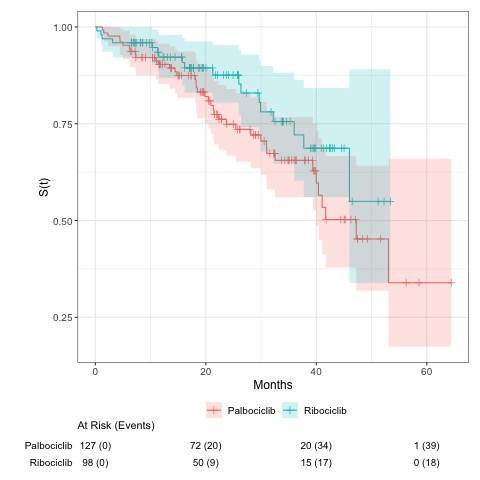
\includegraphics[width=\linewidth]{figures/interest_curve_OS.jpeg}%
%  }%
%  \hfill
%  \subcaptionbox*{(B)}[.44\linewidth]{%
%    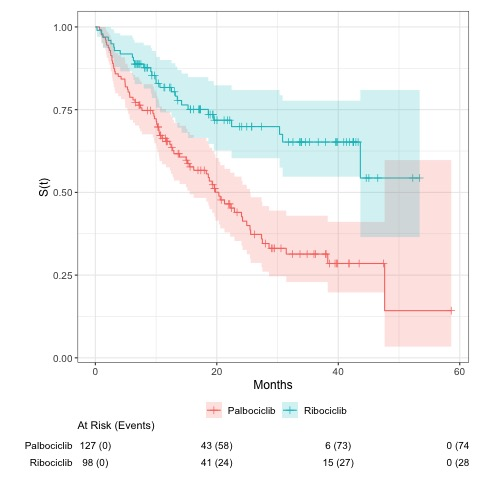
\includegraphics[width=\linewidth]{figures/interest_curve_PFS.jpeg}%
%  }
%\end{figure}

\begin{figure}[ht]
  \caption{Clustering for 3 variables with 3 silos - (A) categorical variables with  proportion with K-Means and (B)  Categorical with K-modes  }\label{fig:interest} 
  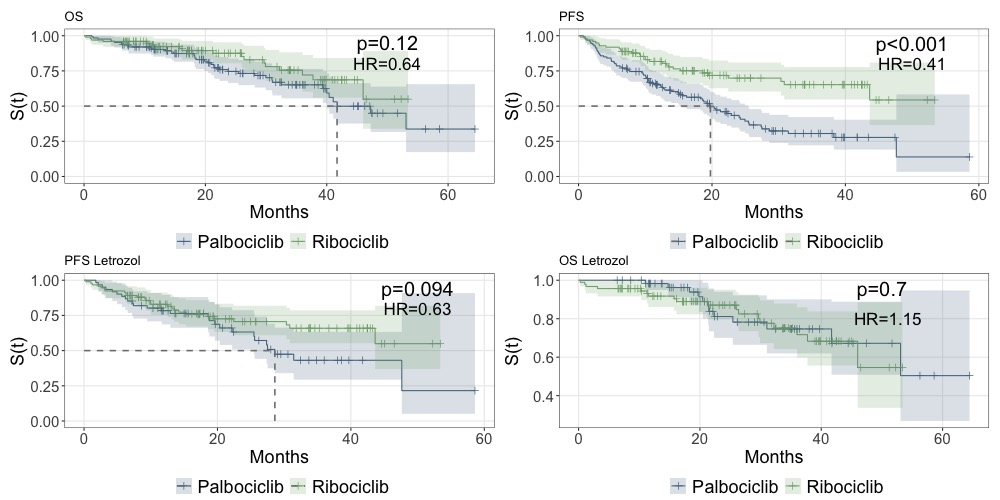
\includegraphics[width=\linewidth]{figures/interest_curve_both.jpeg}%

\end{figure}


\begin{figure}[ht]
  \caption{Clustering for 3 variables with 3 silos - (A) categorical variables with  proportion with K-Means and (B)  Categorical with K-modes  }\label{fig:cox} 
  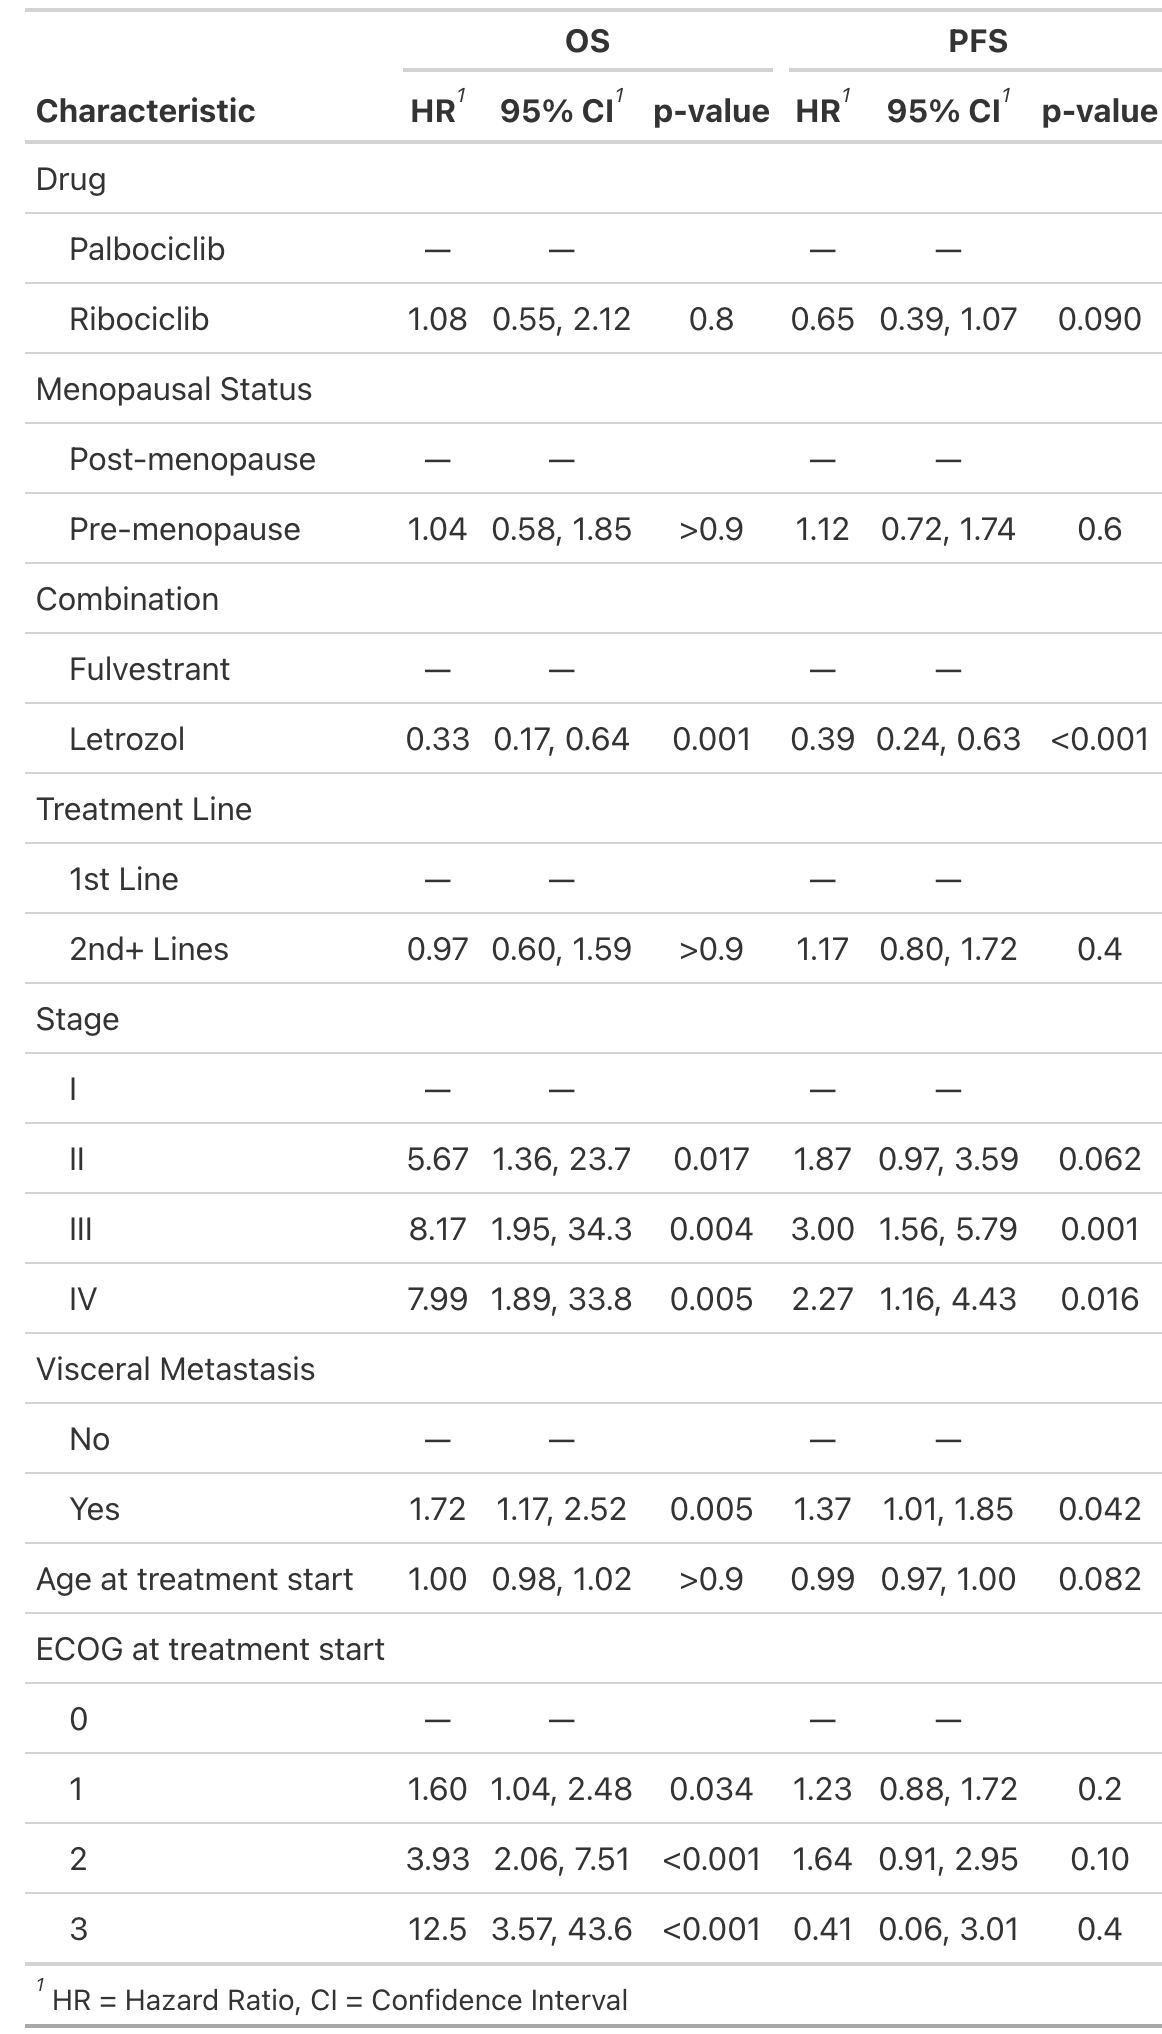
\includegraphics[width=\linewidth]{figures/cox_both.png}%

\end{figure}

\begin{figure}[ht]
  \caption{Clustering for 3 variables with 3 silos - (A) categorical variables with  proportion with K-Means and (B)  Categorical with K-modes  }\label{fig:grouped} 
  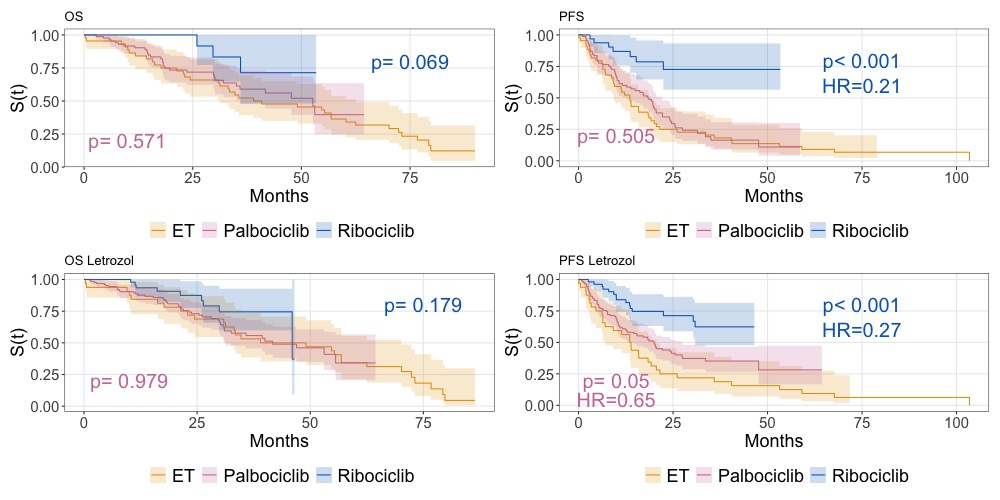
\includegraphics[width=\linewidth]{figures/grouped_curve_both.jpeg}%

\end{figure}

\begin{figure}[ht]
  \caption{Clustering for 3 variables with 3 silos - (A) categorical variables with  proportion with K-Means and (B)  Categorical with K-modes  }\label{fig:propensity} 
  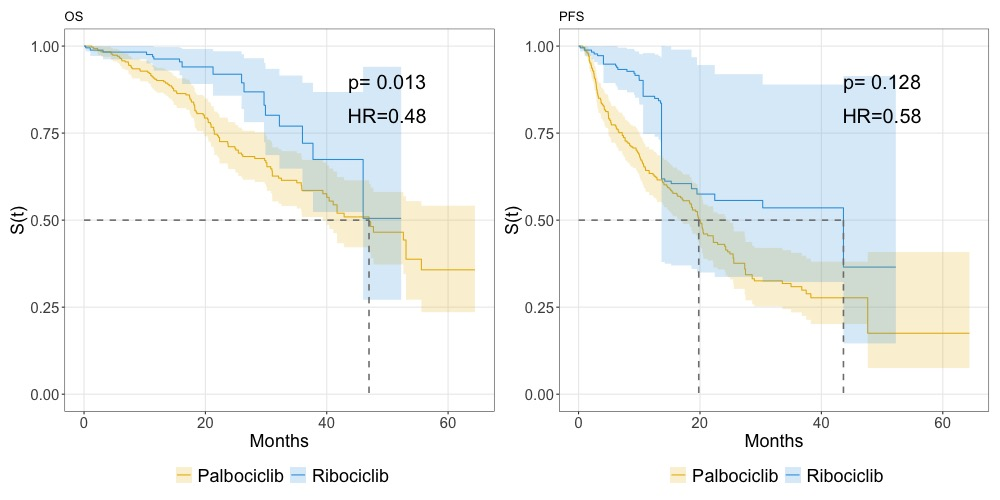
\includegraphics[width=\linewidth]{figures/propensity_score_both.jpeg}%

\end{figure}
